\documentclass[12pt,a4paper]{article}

\usepackage[utf8]{inputenc}
\usepackage[T2A]{fontenc}
\usepackage[ukrainian]{babel}
\usepackage{geometry}
\usepackage{setspace}
\usepackage{array}
\usepackage{longtable}
\usepackage{booktabs}
\usepackage{ragged2e}
\usepackage{indentfirst}
\usepackage{titlesec}
\usepackage{tocloft}
\usepackage{caption}
\usepackage{float}
\usepackage{graphicx}
\usepackage{listings}
\usepackage{xcolor}
\usepackage{pdflscape}

\geometry{
    left=2cm,
    right=2cm,
    top=2cm,
    bottom=2cm
}

\setlength{\emergencystretch}{3em}

\usepackage[
  unicode,
  pdftitle={Курсова робота},
  pdfauthor={Давидчук Артем}
]{hyperref}

\setlength{\parindent}{1.25cm}
\onehalfspacing

\titleformat{\section}
    {\normalfont\bfseries}
    {РОЗДІЛ \thesection.}
    {0.5em}
    {}

\titleformat{\subsection}
    {\normalfont\bfseries}
    {\thesubsection}
    {0.5em}
    {}

\renewcommand{\contentsname}{Зміст}
\renewcommand{\thesection}{\arabic{section}}
\renewcommand{\thesubsection}{\arabic{section}.\arabic{subsection}.}
\renewcommand{\thetable}{\arabic{section}.\arabic{table}}
\renewcommand{\thefigure}{\arabic{section}.\arabic{figure}}
\addto\captionsukrainian{\renewcommand{\tablename}{Таблиця}}
\addto\captionsukrainian{\renewcommand{\figurename}{Рисунок}}
\captionsetup[table]{labelsep=endash,justification=centering}
\captionsetup[figure]{labelsep=endash,justification=centering}
\newcolumntype{C}[1]{>{\centering\arraybackslash}p{#1}}

\makeatletter
\@addtoreset{table}{section}
\@addtoreset{figure}{section}
\makeatother

\lstdefinestyle{plantumlstyle}{
  basicstyle=\ttfamily\small,
  breaklines=true,
  frame=single,
  columns=fullflexible,
  keepspaces=true
}

\begin{document}

\hypersetup{pageanchor=false}
\begin{titlepage}

    \begin{center}
        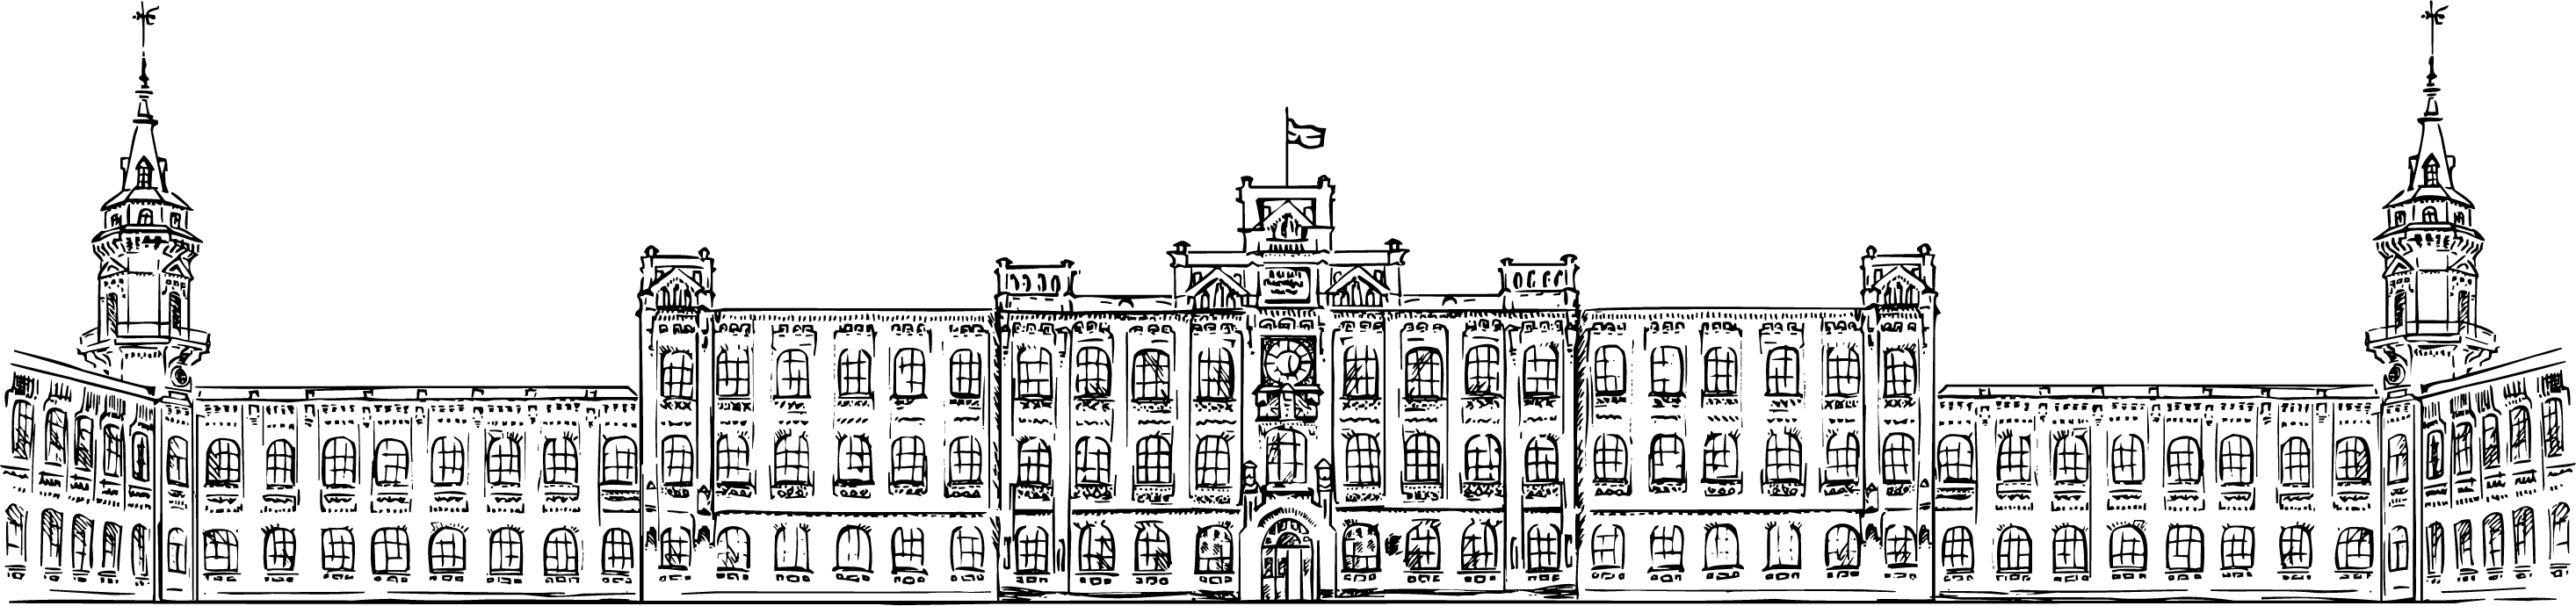
\includegraphics[width=0.7\textwidth]{media/letterhead.png}
    \end{center}

    \begin{center}
        \large Національний технічний університет України\\
        «Київський політехнічний інститут імені Ігоря Сікорського»\\[1em]
        Факультет інформатики та обчислювальної техніки\\
        Кафедра обчислювальної техніки
    \end{center}

    \vfill

    \begin{center}
        \textbf{\LARGE Курсова робота}\\[1em]
        \textbf{\large з дисципліни «Інженерія програмного забезпечення»}\\[1em]
        \textbf{\Large на тему:}\\[0.5em]
        \textbf{\Large «Система діалогової взаємодії з великими мовними моделями з веб- та консольним інтерфейсами»}
    \end{center}

    \vfill

    \begin{flushright}
        Виконав: студент 2 курсу ФІОТ, гр. ІО-41\\
        \textit{Давидчук А. М.}\\
        Залікова книжка № 4106\\[1em]
            Укладач: старший викладач \textit{Васильєва М.\,Д.}
    \end{flushright}

    \vfill

    \begin{center}
        Київ --- 2026
    \end{center}

\end{titlepage}
\hypersetup{pageanchor=true}

\newpage
\section*{ЗАВДАННЯ НА КУРСОВУ РОБОТУ}
\addcontentsline{toc}{section}{ЗАВДАННЯ НА КУРСОВУ РОБОТУ}

\begin{center}
\textbf{Давидчуку Артему Михайловичу}
\end{center}

\begin{enumerate}
  \item \textbf{Тема роботи:} «Система діалогової взаємодії з великими мовними моделями з веб- та консольним інтерфейсами».
  \item \textbf{Термін здачі закінченої роботи:} 13 травня 2026 р.
  \item \textbf{Завдання курсової роботи:} розробити програмну систему для ведення діалогів з локальною великою мовною моделлю, сформувати функціональні та нефункціональні вимоги, спроєктувати архітектуру програмного продукту, реалізувати web- та CLI-інтерфейси, забезпечити збереження історії діалогів у PostgreSQL, реалізувати інтеграцію з локальною LLM, streaming-генерацію, runtime-керування моделлю, підтримку generation presets і LoRA/QLoRA-адаптерів, а також розробити модульні та інтеграційні тести для ключових компонентів системи.
  \item \textbf{Зміст розрахунково-пояснювальної записки:} анотація, вступ, постановка задачі, аналітичний огляд предметної області, проєктування програмного додатку, розробка програмного додатку, тестування програмного додатку, висновки, список використаних джерел.
  \item \textbf{Перелік графічного матеріалу:} діаграма архітектури системи, ER-діаграма бази даних, UML-діаграма прецедентів, UML-діаграма класів, UML-діаграма послідовності надсилання повідомлення.
  \item \textbf{Дата видачі завдання:} лютий 2026 р.
\end{enumerate}

\vspace{1em}

\begin{longtable}{|p{1.2cm}|p{8.3cm}|p{3cm}|p{2.3cm}|}
\caption*{Календарний план виконання курсової роботи}\\
\hline
\textbf{№} & \textbf{Найменування етапу} & \textbf{Термін виконання} & \textbf{Примітка} \\
\hline
1 & Отримання теми та завдання & лютий 2026 & виконано \\
\hline
2 & Підбір та вивчення літератури & лютий 2026 & виконано \\
\hline
3 & Формування технічного завдання & березень 2026 & виконано \\
\hline
4 & Формування вимог до програмної системи & березень 2026 & виконано \\
\hline
5 & Розробка UML-діаграм і архітектури системи & березень 2026 & виконано \\
\hline
6 & Реалізація програмного додатку & квітень 2026 & виконано \\
\hline
7 & Тестування програмного додатку & травень 2026 & виконано \\
\hline
8 & Оформлення пояснювальної записки & травень 2026 & виконано \\
\hline
\end{longtable}

\vspace{1em}

\noindent Студент \hfill \textit{Давидчук А.\,М.}

\vspace{1em}

\noindent Укладач: старший викладач \hfill \textit{Васильєва М.\,Д.}

\newpage
\section*{АНОТАЦІЯ}
\addcontentsline{toc}{section}{АНОТАЦІЯ}

У курсовій роботі розроблено програмну систему діалогової взаємодії з великими мовними моделями. Система призначена для створення та ведення чатів з локальною LLM, збереження історії повідомлень, пошуку по діалогах, експорту чату у Markdown, перемикання локальних моделей і використання LoRA/QLoRA-адаптерів.

Програмний продукт реалізовано мовою Python. Для web-інтерфейсу використано Flask, для збереження даних --- PostgreSQL, для керування міграціями --- Alembic, для запуску локальної мовної моделі --- Hugging Face Transformers. Додатково реалізовано CLI-режим, потокову генерацію відповідей, кнопку зупинки генерації, generation presets, локальний model registry, підтримку математичних формул через KaTeX і підсвічування блоків коду.

У роботі сформовано функціональні та нефункціональні вимоги до системи, виконано аналіз предметної області, спроєктовано багаторівневу архітектуру, ER-діаграму бази даних, UML-діаграми прецедентів, класів і послідовності. Під час реалізації використано принципи ООП, SOLID, розділення відповідальності, Repository/Storage Adapter, Service Layer та Adapter.

Працездатність системи перевірено автоматизованими тестами. Повний набір містить 105 успішних тестів, а покриття production-коду, отримане за допомогою \texttt{coverage.py}, становить 77\%.

\textbf{Ключові слова:} велика мовна модель, LLM, Flask, PostgreSQL, Transformers, LoRA, QLoRA, web-застосунок, CLI, streaming generation, тестування.


\newpage
\section*{ТЕХНІЧНЕ ЗАВДАННЯ}
\addcontentsline{toc}{section}{ТЕХНІЧНЕ ЗАВДАННЯ}

\subsection*{1. Найменування та область використання}

Найменування розробки: система діалогової взаємодії з великими мовними моделями з web- та консольним інтерфейсами. Система може використовуватися як навчальний програмний продукт для демонстрації принципів побудови LLM-застосунків, роботи з локальними мовними моделями, організації persistence-рівня, web-інтерфейсу та автоматизованого тестування.

\subsection*{2. Підстава для розробки}

Підставою для розробки є завдання на виконання курсової роботи з дисципліни «Інженерія програмного забезпечення» для спеціальності 123 «Комп'ютерна інженерія».

\subsection*{3. Мета та призначення розробки}

Метою роботи є розробка програмної системи, яка забезпечує користувачу можливість вести діалог з локальною великою мовною моделлю, зберігати історію чатів, керувати моделями під час виконання програми та перевіряти роботу системи автоматизованими тестами.

Призначення системи:
\begin{itemize}
  \item створення, перегляд, перейменування та видалення чатів;
  \item надсилання повідомлень і отримання відповідей від локальної LLM;
  \item збереження історії діалогів у PostgreSQL;
  \item робота через web-інтерфейс і CLI;
  \item потокове відображення відповіді моделі;
  \item зупинка активної генерації без очікування повного завершення відповіді;
  \item пошук повідомлень і експорт діалогу у Markdown;
  \item відображення Markdown, блоків коду та математичних формул;
  \item перемикання локальних моделей і використання LoRA/QLoRA-адаптерів;
  \item вибір preset-ів генерації та перегляд стану активної моделі;
  \item тестування ключових сценаріїв роботи системи.
\end{itemize}

\subsection*{4. Джерела розробки}

Джерелами розробки є документація Python, Flask, PostgreSQL, Alembic, Hugging Face Transformers, PEFT, pytest, KaTeX, а також матеріали з архітектури програмного забезпечення, UML-моделювання та тестування програмних систем.

\subsection*{5. Технічні вимоги}

\textbf{Вимоги до програмного продукту:}
\begin{itemize}
  \item система повинна мати web-інтерфейс для роботи з чатами;
  \item система повинна підтримувати CLI-режим;
  \item система повинна зберігати історію чатів і повідомлень;
  \item система повинна підтримувати локальний LLM-backend;
  \item система повинна дозволяти перемикати локальні моделі під час роботи;
  \item система повинна підтримувати streaming generation;
  \item система повинна дозволяти зупиняти активну генерацію;
  \item система повинна підтримувати пошук повідомлень у чатах;
  \item система повинна підтримувати експорт діалогу у Markdown;
  \item система повинна відображати Markdown, блоки коду та математичні формули;
  \item система повинна показувати активний backend, модель, adapter і preset генерації;
  \item система повинна підтримувати generation presets;
  \item система повинна підтримувати підключення LoRA/QLoRA-адаптерів через конфігураційний файл;
  \item система повинна контрольовано повідомляти про помилки завантаження моделі або adapter-а;
  \item система повинна мати автоматизовані тести для основної бізнес-логіки.
\end{itemize}

\textbf{Вимоги до програмного забезпечення:}
\begin{itemize}
  \item Python 3.10 або вище;
  \item PostgreSQL;
  \item Flask;
  \item Hugging Face Transformers;
  \item PEFT для підключення LoRA/QLoRA-адаптерів;
  \item Alembic;
  \item pytest і coverage.py;
  \item KaTeX для відображення математичних формул у web-інтерфейсі.
\end{itemize}

\textbf{Вимоги до апаратної частини:}
\begin{itemize}
  \item персональний комп'ютер або ноутбук, здатний запускати Python-застосунок;
  \item достатній обсяг оперативної пам'яті для запуску обраної локальної LLM;
  \item достатній обсяг дискового простору для збереження локальних моделей і adapter-ів;
  \item GPU є бажаним для швидшої генерації, але система може працювати і на CPU з малими моделями.
\end{itemize}

\subsection*{6. Етапи розробки}

Основними етапами розробки є отримання теми, вивчення джерел, формування вимог, проєктування архітектури та UML-діаграм, реалізація програмного продукту, тестування, оформлення пояснювальної записки та підготовка до захисту.


\tableofcontents
\newpage

\section*{ВСТУП}
\addcontentsline{toc}{section}{ВСТУП}

Сучасний розвиток програмних систем дедалі частіше пов'язаний з інтеграцією засобів штучного інтелекту, зокрема великих мовних моделей. Такі моделі використовуються для побудови діалогових асистентів, автоматизованого пояснення навчального матеріалу, генерації програмного коду, аналізу текстів та підтримки користувача під час роботи з інформаційними системами. Водночас практичне використання LLM потребує не лише самої моделі, а й прикладного програмного середовища, яке забезпечує введення запитів, збереження історії діалогів, відображення відповідей, керування параметрами генерації та обробку помилок.

Актуальність теми курсової роботи зумовлена необхідністю створення навчальної програмної системи, яка демонструє повний цикл взаємодії користувача з локальною великою мовною моделлю. На відміну від готових хмарних сервісів, власна реалізація дозволяє дослідити архітектуру такої системи, організацію web- та CLI-інтерфейсів, роботу зі сховищем даних, інтеграцію локальної pretrained-моделі, потокову генерацію відповідей та розширення через LoRA/QLoRA-адаптери.

Метою курсової роботи є розробка програмної системи діалогової взаємодії з великими мовними моделями з підтримкою web- та консольного інтерфейсів, збереженням історії діалогів у PostgreSQL та можливістю запуску локальних моделей через Hugging Face Transformers.

Для досягнення поставленої мети необхідно виконати такі завдання:
\begin{enumerate}
  \item проаналізувати предметну область діалогових систем на основі LLM;
  \item розглянути існуючі рішення та визначити їхні переваги й обмеження;
  \item сформувати функціональні та нефункціональні вимоги до системи;
  \item спроєктувати архітектуру програмного продукту та структуру бази даних;
  \item реалізувати web-інтерфейс для роботи з чатами та повідомленнями;
  \item реалізувати CLI-режим роботи;
  \item організувати збереження даних у PostgreSQL з використанням міграцій;
  \item інтегрувати локальний LLM-backend на основі Transformers;
  \item реалізувати runtime-перемикання моделей, streaming generation, зупинку генерації та підтримку LoRA/QLoRA-адаптерів;
  \item виконати тестування основних модулів системи.
\end{enumerate}

Об'єктом дослідження є процес побудови програмних систем для діалогової взаємодії користувача з великими мовними моделями.

Предметом дослідження є архітектурні, програмні та інтерфейсні засоби реалізації локальної LLM-системи з web- та CLI-режимами, базою даних PostgreSQL і локальним inference-backend.

Практичне значення роботи полягає у створенні працездатного програмного продукту, який може використовуватися як навчальний приклад побудови модульної LLM-системи, а також як основа для подальших експериментів з локальними моделями, адаптерами, параметрами генерації та розширенням функціональності.

\newpage

\section{АНАЛІТИЧНИЙ ОГЛЯД ПРЕДМЕТНОЇ ОБЛАСТІ}

\subsection{Характеристика предметної області діалогових систем на основі великих мовних моделей}

Сучасні програмні системи дедалі частіше використовують засоби штучного інтелекту для автоматизованої обробки текстової інформації, підтримки користувача, генерації відповідей, пояснення навчального матеріалу, написання програмного коду та організації діалогової взаємодії. Одним із найбільш поширених напрямів розвитку таких систем є використання великих мовних моделей, або Large Language Models (LLM).

Великі мовні моделі --- це програмні компоненти, побудовані на основі нейронних мереж, які здатні обробляти природну мову, аналізувати контекст запиту та генерувати текстові відповіді. У прикладних системах LLM зазвичай не використовуються ізольовано: навколо моделі створюється програмна інфраструктура, яка забезпечує введення повідомлень користувача, передавання запиту до моделі, отримання відповіді, збереження історії діалогу та відображення результату в зручному інтерфейсі.

Предметна область даної курсової роботи охоплює розробку програмної системи для діалогової взаємодії з великою мовною моделлю. Така система повинна забезпечувати користувачу можливість створювати окремі діалоги, надсилати повідомлення, отримувати відповіді від мовної моделі, переглядати історію листування та працювати з програмою як через веб-інтерфейс, так і через консольний режим.

Особливістю обраної предметної області є поєднання кількох напрямів програмної інженерії:
\begin{itemize}
  \item побудова користувацького інтерфейсу для діалогової взаємодії;
  \item організація бізнес-логіки керування чатами та повідомленнями;
  \item інтеграція pretrained-моделі через окремий LLM-backend;
  \item збереження історії діалогів у реляційній базі даних PostgreSQL;
  \item створення модульної архітектури, що дозволяє надалі підключати інші моделі або адаптери;
  \item забезпечення тестованості основних компонентів системи.
\end{itemize}

Розроблювана система орієнтована на локальне або навчально-дослідницьке використання. На відміну від багатьох хмарних сервісів, вона передбачає можливість запуску на персональному комп'ютері, використання локально завантажених pretrained-моделей та контроль над структурою програмного продукту.

\subsection{Аналіз підходів до побудови програмних систем для взаємодії з LLM}

Побудова LLM-системи може виконуватися різними способами. Найпростішим варіантом є використання готового хмарного сервісу, де користувач взаємодіє з моделлю через браузер або API. Такий підхід мінімізує складність розгортання, але зменшує контроль над моделлю, способом збереження даних і внутрішньою архітектурою.

Інший підхід полягає у використанні локальних інструментів для запуску open-source або open-weight моделей. У цьому випадку модель завантажується на комп'ютер користувача, а генерація відповідей виконується локально. Перевагою такого підходу є більший контроль над даними та можливість експериментувати з різними моделями. Недоліком є залежність від апаратних ресурсів комп'ютера.

Третій підхід --- створення власної прикладної системи, яка інтегрує LLM як один із модулів. У цьому випадку мовна модель є не самостійним продуктом, а частиною програмної архітектури. Саме цей підхід обрано в даній курсовій роботі. Він дозволяє відокремити користувацький інтерфейс, бізнес-логіку, сховище даних і LLM-backend.

\subsection{Огляд існуючих аналогів і подібних програмних рішень}

Для визначення доцільності розробки власної системи було розглянуто декілька існуючих програмних рішень, пов'язаних із діалоговою взаємодією з LLM: ChatGPT, Claude, Google Gemini, LM Studio, Ollama та Open WebUI.

ChatGPT, Claude та Google Gemini є хмарними діалоговими сервісами, які надають користувачу зручний web-інтерфейс і високу якість відповідей. Однак такі системи не дають повного контролю над моделлю, способом збереження історії та внутрішньою архітектурою.

LM Studio та Ollama орієнтовані на локальний запуск моделей. Вони спрощують роботу з pretrained-моделями, але не є навчальними програмними системами, у яких користувач самостійно проєктує web-рівень, CLI-рівень, бізнес-логіку, сховище даних і LLM-backend.

Open WebUI є self-hosted web-інтерфейсом для взаємодії з LLM-backend-ами. Це функціонально близьке рішення, однак воно є готовою платформою, тоді як у даній курсовій роботі важливим є проєктування та реалізація власної модульної системи.

\subsection{Порівняльний аналіз існуючих рішень}

Порівняльний аналіз аналогів наведено в таблиці~\ref{tab:llm-analogues}.

\begin{landscape}
\small
\begin{longtable}{|p{3.2cm}|p{3.8cm}|C{2.4cm}|C{1.7cm}|C{1.7cm}|C{2.0cm}|p{3.4cm}|}
\caption{Порівняння існуючих рішень для діалогової взаємодії з LLM}
\label{tab:llm-analogues}\\
\hline
\textbf{Рішення} & \textbf{Тип системи} & \textbf{Локальний запуск} & \textbf{Web} & \textbf{CLI} & \textbf{Власна БД} & \textbf{Навчальне розширення} \\
\hline
\endfirsthead
\hline
\textbf{Рішення} & \textbf{Тип системи} & \textbf{Локальний запуск} & \textbf{Web} & \textbf{CLI} & \textbf{Власна БД} & \textbf{Навчальне розширення} \\
\hline
\endhead
ChatGPT & Хмарний сервіс & Ні & Так & Ні & Ні & Обмежене \\
\hline
Claude & Хмарний сервіс & Ні & Так & Ні & Ні & Обмежене \\
\hline
Google Gemini & Хмарний сервіс & Ні & Так & Ні & Ні & Обмежене \\
\hline
LM Studio & Локальний застосунок & Так & Так & Частково & Обмежено & Обмежене \\
\hline
Ollama & Локальний LLM-runner & Так & Ні / через сторонні UI & Так & Ні & Середнє \\
\hline
Open WebUI & Self-hosted web UI & Через backend & Так & Ні & Так & Середнє \\
\hline
Розроблювана система & Навчальна модульна LLM-система & Так & Так & Так & Так, PostgreSQL & Високе \\
\hline
\end{longtable}
\normalsize
\end{landscape}

\subsection{Недоліки існуючих рішень та обґрунтування необхідності власної розробки}

Аналіз аналогів показує, що існуючі рішення мають низку обмежень у контексті навчальної розробки LLM-системи. Хмарні сервіси не дозволяють повністю контролювати модель, механізм її запуску та структуру збереження діалогів. Локальні інструменти для запуску моделей часто зосереджені саме на інференсі, але не завжди забезпечують навчально корисну архітектуру з чітким поділом на web-рівень, CLI-рівень, бізнес-логіку, storage-рівень і LLM-рівень.

Тому розробка власної системи є обґрунтованою. Вона дозволяє реалізувати програмний продукт, який поєднує web-інтерфейс, консольний режим, збереження історії в PostgreSQL, LLM-backend із підтримкою локальної pretrained-моделі, runtime-керування моделлю, потокову генерацію відповідей та основу для подальшого розширення через LoRA/QLoRA-адаптацію.

\subsection{Постановка задачі розробки програмної системи}

Метою розробки є створення програмної системи для діалогової взаємодії з великою мовною моделлю з підтримкою web- та консольного інтерфейсів.

Для досягнення поставленої мети необхідно розв'язати такі задачі:
\begin{enumerate}
  \item Розробити структуру програмного застосунку з головним файлом запуску \texttt{app.py}.
  \item Реалізувати web-інтерфейс для створення, вибору, перейменування та видалення чатів.
  \item Реалізувати консольний режим роботи для взаємодії з чатами через командний рядок.
  \item Реалізувати модуль керування чатами та повідомленнями.
  \item Організувати збереження історії чатів і повідомлень у PostgreSQL.
  \item Реалізувати LLM-backend із можливістю використання pretrained-моделі через Hugging Face Transformers.
  \item Забезпечити підтримку локально завантаженої instruction-моделі.
  \item Додати відображення Markdown, блоків коду та математичних формул у web-інтерфейсі.
  \item Реалізувати автоматизовані тести для основних компонентів системи.
  \item Реалізувати підтримку LoRA/QLoRA-адаптерів для локальних моделей.
\end{enumerate}

\newpage

\section{ПРОЄКТУВАННЯ СИСТЕМИ ДІАЛОГОВОЇ ВЗАЄМОДІЇ З LLM}

\subsection{Вибір архітектури програмної системи}

Для розробки системи діалогової взаємодії з LLM обрано модульну багаторівневу архітектуру. Такий підхід дозволяє розділити відповідальність між окремими компонентами системи та забезпечити можливість подальшого розширення без істотної зміни існуючого коду.

Загальна архітектура системи складається з таких рівнів:
\begin{itemize}
  \item рівень користувацької взаємодії;
  \item рівень бізнес-логіки;
  \item рівень збереження даних;
  \item рівень взаємодії з мовною моделлю;
  \item рівень конфігурації та допоміжних сервісів.
\end{itemize}

Рівень користувацької взаємодії представлений web-інтерфейсом і CLI-режимом. Рівень бізнес-логіки реалізовано у компоненті \texttt{ChatManager}. Рівень збереження даних реалізовано через \texttt{PostgresStorage}, а рівень взаємодії з мовною моделлю --- через \texttt{BaseLLMService}, \texttt{TransformersLLMService}, \texttt{UnavailableLLMService} та \texttt{LLMRuntime}.

\begin{figure}[H]
\centering
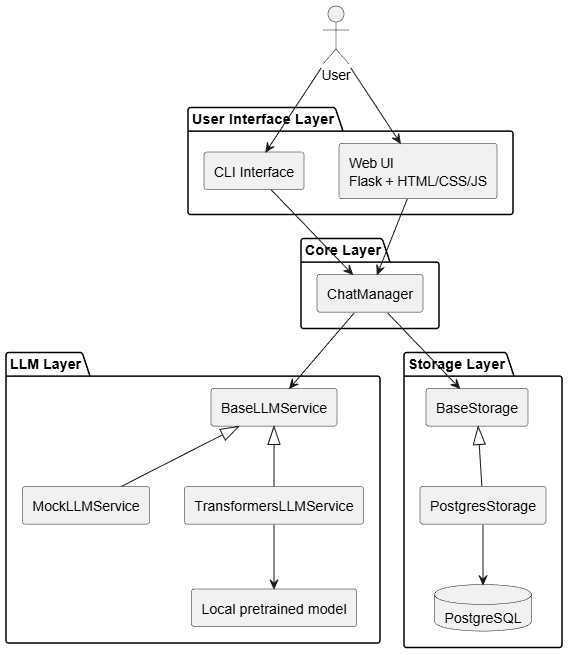
\includegraphics[width=0.8\textwidth]{media/architecture.png}
\caption{Загальна архітектура системи}
\label{fig:architecture}
\end{figure}

\subsection{Формування функціональних і нефункціональних вимог}

На основі технічного завдання та аналізу предметної області сформовано функціональні та нефункціональні вимоги до системи.

\begin{longtable}{|p{1.5cm}|p{13.5cm}|}
\caption{Функціональні вимоги до системи}
\label{tab:functional-requirements}\\
\hline
\textbf{Код} & \textbf{Вимога} \\
\hline
\endfirsthead
\hline
\textbf{Код} & \textbf{Вимога} \\
\hline
\endhead
F1 & Система повинна запускатися з головного файла \texttt{app.py}. \\
\hline
F2 & Система повинна підтримувати web-режим роботи. \\
\hline
F3 & Система повинна підтримувати CLI-режим роботи через параметр \texttt{-t}. \\
\hline
F4 & Користувач повинен мати можливість створювати новий чат. \\
\hline
F5 & Користувач повинен мати можливість відкривати наявний чат. \\
\hline
F6 & Користувач повинен мати можливість перейменовувати чат. \\
\hline
F7 & Користувач повинен мати можливість видаляти чат. \\
\hline
F8 & Користувач повинен мати можливість надсилати повідомлення. \\
\hline
F9 & Система повинна генерувати відповідь через підключений LLM-backend. \\
\hline
F10 & Система повинна зберігати історію чатів і повідомлень у PostgreSQL. \\
\hline
F11 & Система повинна коректно повідомляти про помилки завантаження моделі. \\
\hline
F12 & Система повинна підтримувати Transformers-backend для локальної pretrained-моделі. \\
\hline
F13 & Система повинна відображати Markdown, блоки коду та математичні формули у відповідях асистента. \\
\hline
F14 & Система повинна показувати активний LLM-backend, назву моделі та preset генерації. \\
\hline
F15 & Система повинна підтримувати runtime-перемикання та вивантаження локальних моделей. \\
\hline
F16 & Система повинна підтримувати streaming generation і зупинку активної генерації. \\
\hline
F17 & Система повинна підтримувати підключення PEFT LoRA/QLoRA-адаптерів. \\
\hline
F18 & Система повинна підтримувати пошук повідомлень і експорт діалогу у Markdown. \\
\hline
\end{longtable}

\begin{longtable}{|p{1.5cm}|p{13.5cm}|}
\caption{Нефункціональні вимоги до системи}
\label{tab:non-functional-requirements}\\
\hline
\textbf{Код} & \textbf{Вимога} \\
\hline
\endfirsthead
\hline
\textbf{Код} & \textbf{Вимога} \\
\hline
\endhead
NF1 & Архітектура системи повинна бути модульною: web-рівень, CLI-рівень, доменна логіка, сховище даних, LLM-рівень і конфігурація мають бути винесені в окремі модулі. \\
\hline
NF2 & Компоненти системи повинні мати слабке зв'язування через абстракції \texttt{BaseStorage} і \texttt{BaseLLMService}; доменна логіка не повинна напряму залежати від Flask, PostgreSQL або Transformers. \\
\hline
NF3 & Система повинна бути придатною до подальшого розширення: додавання нового storage-backend, LLM-backend або конфігурації моделі не повинно вимагати зміни основної логіки \texttt{ChatManager}. \\
\hline
NF4 & Основна бізнес-логіка повинна бути покрита автоматизованими тестами на рівні не менше 70\% production-коду; фактичне покриття становить 77\%, набір тестів містить 105 перевірок. \\
\hline
NF5 & Система повинна коректно обробляти помилки користувача: порожні повідомлення, некоректні або дубльовані назви чатів, відсутні моделі та помилки адаптерів мають повертати контрольоване повідомлення, а не аварійне завершення. \\
\hline
NF6 & Web-інтерфейс повинен бути зручним і зрозумілим: користувач має бачити активний backend, модель, adapter, preset генерації, стан завантаження моделі, кнопку зупинки генерації та кнопки копіювання для блоків коду. \\
\hline
NF7 & Дані чатів повинні зберігатися у структурованому вигляді в таблицях \texttt{chats} і \texttt{messages} з ідентифікаторами чатів, ролями повідомлень, timestamp-ами та порядковим номером повідомлення. \\
\hline
NF8 & Конфігурація системи повинна виконуватися через змінні середовища або \texttt{.env} файл; паролі, локальні моделі та адаптери не повинні додаватися до Git-репозиторію. \\
\hline
NF9 & Система не повинна жорстко залежати від конкретної мовної моделі: доступні моделі мають визначатися через локальний каталог \texttt{models/}, \texttt{model\_config.json}, runtime-перемикання та generation presets. \\
\hline
NF10 & Система повинна підтримувати роботу на персональному комп'ютері з Python 3.10 або вище, PostgreSQL і локальними model artifacts; для великих моделей може використовуватися GPU, але малі моделі можуть запускатися на CPU. \\
\hline
\end{longtable}

\subsection{Матриця трасування вимог}

Для підтвердження повноти реалізації сформовано матрицю трасування, яка пов'язує вимоги з програмними модулями та способом перевірки. Такий підхід дозволяє показати, що функціональні й нефункціональні вимоги не є декларативними, а мають відповідні елементи реалізації та тестування.

\small
\begin{longtable}{|p{2.2cm}|p{5.2cm}|p{7.2cm}|}
\caption{Матриця трасування вимог}
\label{tab:requirements-traceability}\\
\hline
\textbf{Вимога} & \textbf{Модуль реалізації} & \textbf{Перевірка} \\
\hline
\endfirsthead
\hline
\textbf{Вимога} & \textbf{Модуль реалізації} & \textbf{Перевірка} \\
\hline
\endhead
F1--F3 & \texttt{app.py}, \texttt{src/web}, \texttt{src/cli} & Перевірка запуску web-режиму, CLI-режиму та тестування базових web routes. \\
\hline
F4--F8 & \texttt{ChatManager}, web endpoints, storage-рівень & Тести \texttt{chat\_manager} і \texttt{web\_app}: створення, відкриття, перейменування, видалення чатів і надсилання повідомлень. \\
\hline
F9--F12 & \texttt{BaseLLMService}, \texttt{TransformersLLMService}, \texttt{UnavailableLLMService}, \texttt{LLMRuntime} & Тести runtime-станів, побудови prompt-ів, fallback-поведінки та обробки помилок завантаження моделі. \\
\hline
F13 & HTML-шаблони, \texttt{script.js}, Markdown/KaTeX renderer & Ручна browser-перевірка Markdown, code blocks і формул, а також regression-перевірки web-відображення. \\
\hline
F14--F17 & \texttt{LLMRuntime}, \texttt{model\_registry}, \texttt{model\_config.json}, generation presets, PEFT adapter loading & Тести \texttt{llm\_runtime}, \texttt{model\_registry}, \texttt{config\_presets}, \texttt{transformers\_prompting}. \\
\hline
F18 & \texttt{ChatManager}, routes пошуку та експорту & Тести пошуку повідомлень і експорту Markdown у групах \texttt{chat\_manager} та \texttt{web\_app}. \\
\hline
NF1--NF3 & Поділ на \texttt{src/core}, \texttt{src/storage}, \texttt{src/llm}, \texttt{src/web}, \texttt{src/cli} & Перевірка структури коду, використання абстракцій і можливість підстановки fake-реалізацій у тестах. \\
\hline
NF4 & Набір автоматизованих тестів, \texttt{coverage.py} & 105 успішних тестів, production coverage 77\%. \\
\hline
NF5--NF8 & Валідація у \texttt{ChatManager}, web routes, storage factory, \texttt{src/config.py} & Тести помилкових сценаріїв, конфігурації, Alembic-міграцій і storage factory. \\
\hline
NF9--NF10 & \texttt{model\_registry}, runtime-перемикання, локальні model artifacts & Перевірка сканування моделей, читання \texttt{model\_config.json}, перемикання і вивантаження моделей. \\
\hline
\end{longtable}
\normalsize

\subsection{Проєктування основних функціональних модулів}

Програмну систему поділено на такі основні модулі: web-інтерфейс, CLI-інтерфейс, модуль керування чатами, LLM-backend, runtime-керування моделлю, модуль збереження даних і конфігураційний модуль.

Модуль web-інтерфейсу відповідає за взаємодію користувача із системою через браузер. CLI-модуль забезпечує альтернативний текстовий режим роботи. Модуль \texttt{ChatManager} координує операції між інтерфейсами користувача, сховищем даних і LLM-сервісом. LLM-модуль реалізує генерацію відповідей через локальну pretrained-модель. Runtime-модуль керує станом моделі, завантаженням, вивантаженням, streaming-генерацією та зупинкою генерації. Модуль збереження даних використовує PostgreSQL для збереження чатів і повідомлень.

\subsection{Проєктування структури бази даних}

Для збереження історії діалогів використовується реляційна база даних PostgreSQL. Структура бази даних складається з двох основних таблиць: \texttt{chats} і \texttt{messages}.

\begin{longtable}{|p{4cm}|p{4cm}|p{7cm}|}
\caption{Структура таблиці \texttt{chats}}
\label{tab:chats-table}\\
\hline
\textbf{Поле} & \textbf{Тип} & \textbf{Опис} \\
\hline
\endfirsthead
\hline
\textbf{Поле} & \textbf{Тип} & \textbf{Опис} \\
\hline
\endhead
\texttt{id} & TEXT & Унікальний ідентифікатор чату \\
\hline
\texttt{title} & TEXT & Назва чату \\
\hline
\texttt{created\_at} & TIMESTAMPTZ & Дата і час створення чату \\
\hline
\texttt{updated\_at} & TIMESTAMPTZ & Дата і час останнього оновлення чату \\
\hline
\end{longtable}

\begin{longtable}{|p{4cm}|p{4cm}|p{7cm}|}
\caption{Структура таблиці \texttt{messages}}
\label{tab:messages-table}\\
\hline
\textbf{Поле} & \textbf{Тип} & \textbf{Опис} \\
\hline
\endfirsthead
\hline
\textbf{Поле} & \textbf{Тип} & \textbf{Опис} \\
\hline
\endhead
\texttt{id} & BIGSERIAL & Унікальний ідентифікатор повідомлення \\
\hline
\texttt{chat\_id} & TEXT & Ідентифікатор чату, до якого належить повідомлення \\
\hline
\texttt{role} & TEXT & Роль автора повідомлення: \texttt{user} або \texttt{assistant} \\
\hline
\texttt{content} & TEXT & Текст повідомлення \\
\hline
\texttt{timestamp} & TIMESTAMPTZ & Дата і час створення повідомлення \\
\hline
\texttt{position} & INTEGER & Порядковий номер повідомлення в чаті \\
\hline
\end{longtable}

\begin{figure}[H]
\centering
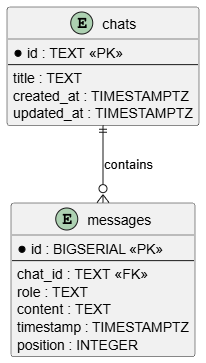
\includegraphics[width=0.5\textwidth]{media/database_er.png}
\caption{ER-діаграма бази даних}
\label{fig:database-er}
\end{figure}

\subsection{UML-діаграма прецедентів}

\begin{figure}[H]
\centering
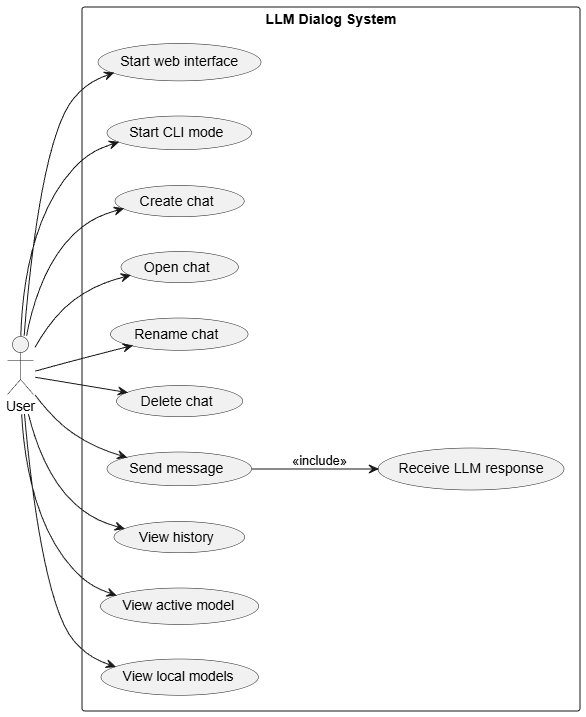
\includegraphics[width=0.8\textwidth]{media/use_case.png}
\caption{UML-діаграма прецедентів системи}
\label{fig:use-case}
\end{figure}

\subsection{UML-діаграма класів}

\begin{figure}[H]
\centering
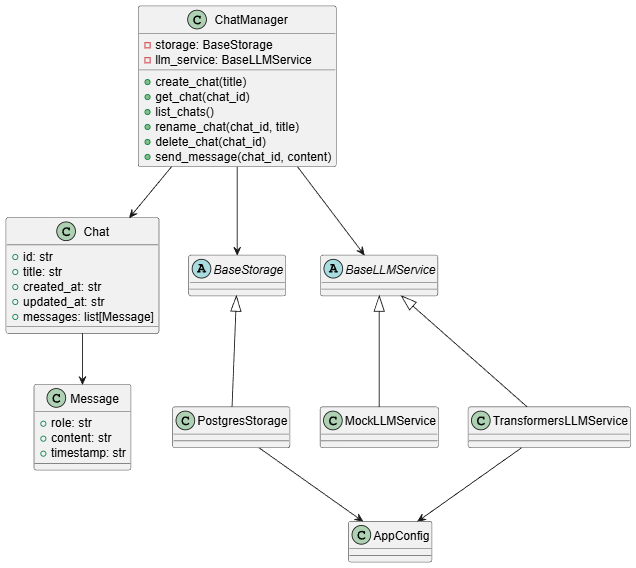
\includegraphics[width=\textwidth]{media/class_diagram.png}
\caption{UML-діаграма класів системи}
\label{fig:class-diagram}
\end{figure}

\subsection{UML-діаграма послідовності}

\begin{figure}[H]
\centering
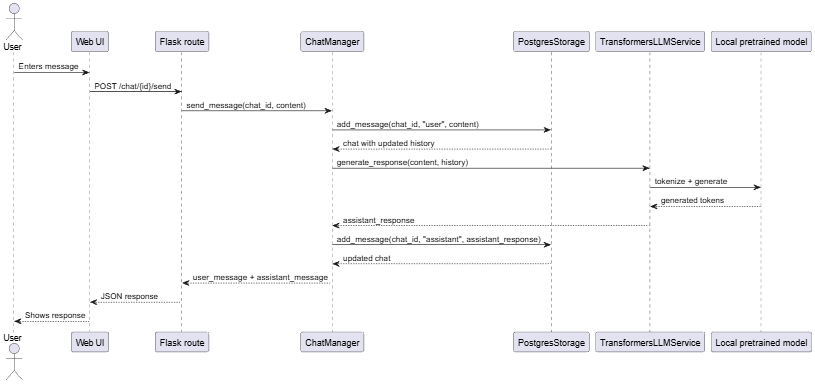
\includegraphics[width=\textwidth]{media/sequence_send_message.png}
\caption{UML-діаграма послідовності надсилання повідомлення}
\label{fig:sequence-send-message}
\end{figure}

\subsection{Опис логічної структури системи}

Логічна структура системи побудована так, щоб окремі частини програмного продукту мали чітко визначені обов'язки. Web-інтерфейс і CLI-інтерфейс не працюють безпосередньо з базою даних або моделлю. Вони звертаються до \texttt{ChatManager}, який координує виконання операцій.

\texttt{ChatManager} не залежить від конкретної реалізації LLM-рівня. Для генерації відповідей використовується інтерфейс \texttt{BaseLLMService}. Для збереження даних у поточній реалізації використовується \texttt{PostgresStorage}, що працює з PostgreSQL.

PostgreSQL використовується як основне сховище даних. Це дозволяє зберігати історію діалогів у структурованому вигляді, підтримувати зв'язок між чатами й повідомленнями та надалі розширювати схему бази даних.

LLM-рівень підтримує Transformers-режим, який дозволяє підключати pretrained-модель, завантажену в локальну директорію \texttt{models/}. Якщо модель не може бути завантажена, використовується \texttt{UnavailableLLMService}, що зберігає інформацію про помилку та дозволяє відобразити її у web-інтерфейсі. Система реалізує потокову генерацію відповідей, зупинку генерації, runtime-перемикання моделей без перезапуску застосунку та підключення LoRA/QLoRA-адаптерів.

Конфігурація системи виконується через змінні середовища або \texttt{.env} файл. Це дозволяє змінювати LLM-backend, модель, preset генерації та параметри підключення до PostgreSQL без зміни вихідного коду.

Таким чином, обрана структура забезпечує модульність, розширюваність, зручність тестування та відповідність поставленим вимогам до курсового проєкту.

\newpage

\section{РЕАЛІЗАЦІЯ, ТЕСТУВАННЯ ТА ЕКСПЛУАТАЦІЯ ПРОГРАМНОЇ СИСТЕМИ}

\subsection{Загальна структура програмної реалізації}

Програмну систему реалізовано мовою Python з використанням Flask для web-рівня, PostgreSQL для збереження даних, Alembic для керування міграціями бази даних та Hugging Face Transformers для запуску локальної мовної моделі. Вихідний код розділено на окремі модулі відповідно до їхньої відповідальності.

Головним файлом запуску є \texttt{app.py}. Він аналізує параметри командного рядка і запускає один із двох режимів роботи:
\begin{itemize}
  \item web-режим, у якому створюється Flask-застосунок;
  \item CLI-режим, який активується параметром \texttt{-t} або \texttt{--terminal}.
\end{itemize}

Основні каталоги програмної системи наведено у таблиці~\ref{tab:project-structure}.

\small
\begin{longtable}{|p{4.2cm}|p{10.2cm}|}
\caption{Структура програмної реалізації}
\label{tab:project-structure}\\
\hline
\textbf{Каталог або файл} & \textbf{Призначення} \\
\hline
\endfirsthead
\hline
\textbf{Каталог або файл} & \textbf{Призначення} \\
\hline
\endhead
\texttt{app.py} & Головна точка входу, вибір web- або CLI-режиму. \\
\hline
\texttt{src/core} & Доменні моделі та менеджер чатів. \\
\hline
\texttt{src/web} & Flask routes, HTML-шаблони, CSS і JavaScript web-інтерфейсу. \\
\hline
\texttt{src/cli} & Реалізація консольного режиму. \\
\hline
\texttt{src/storage} & Абстракція сховища та PostgreSQL-реалізація. \\
\hline
\texttt{src/llm} & Інтерфейс LLM-сервісу, runtime-керування моделлю та Transformers-backend. \\
\hline
\texttt{migrations} & Alembic-міграції схеми бази даних. \\
\hline
\texttt{scripts} & Допоміжні скрипти для завантаження моделей, адаптерів і експериментального fine-tuning. \\
\hline
\texttt{tests} & Автоматизовані тести системи. \\
\hline
\end{longtable}
\normalsize

Такий поділ дозволяє відокремити інтерфейс користувача від бізнес-логіки, сховища даних та LLM-рівня. Це спрощує тестування, підтримку та подальший розвиток системи.

\subsection{Реалізація доменної логіки}

Доменний рівень системи реалізовано у модулі \texttt{src/core}. Основними сутностями є \texttt{Chat}, \texttt{Message} та \texttt{SearchResult}. Вони описують чат, окреме повідомлення та результат пошуку відповідно.

Клас \texttt{ChatManager} є центральним сервісом прикладної логіки. Він не залежить безпосередньо від Flask, PostgreSQL або Transformers, а працює через абстракції \texttt{BaseStorage} та \texttt{BaseLLMService}. Завдяки цьому один і той самий менеджер використовується як у web-інтерфейсі, так і в CLI-режимі.

Основні можливості \texttt{ChatManager}:
\begin{itemize}
  \item створення чатів з унікальними назвами;
  \item перевірка назв чатів на порожнє значення, довжину та дублювання;
  \item отримання списку чатів;
  \item додавання повідомлень користувача й асистента;
  \item генерація відповіді через підключений LLM-сервіс;
  \item streaming-генерація з подальшим збереженням фінальної відповіді;
  \item пошук повідомлень;
  \item перейменування та видалення чатів.
\end{itemize}

При надсиланні повідомлення \texttt{ChatManager} спочатку зберігає повідомлення користувача, формує історію діалогу, передає її до LLM-сервісу, отримує відповідь і зберігає її як повідомлення асистента. Такий підхід забезпечує цілісність історії діалогу та дозволяє моделі враховувати контекст поточного чату.

\subsection{Застосовані принципи проєктування та патерни}

Під час реалізації системи було використано об'єктно-орієнтований підхід з розділенням відповідальності між окремими класами та модулями. Доменні сутності \texttt{Chat}, \texttt{Message} і \texttt{SearchResult} описують основні об'єкти предметної області, а сервіс \texttt{ChatManager} інкапсулює бізнес-логіку роботи з діалогами.

Основні принципи проєктування, використані у системі:
\begin{itemize}
  \item \textbf{Single Responsibility}. Кожен основний компонент має окрему зону відповідальності: \texttt{ChatManager} керує сценаріями чатів, \texttt{PostgresStorage} відповідає за збереження даних, \texttt{TransformersLLMService} інкапсулює роботу з локальною моделлю, а \texttt{LLMRuntime} керує станом завантаженої моделі.
  \item \textbf{Dependency Inversion}. Доменна логіка залежить не від конкретної PostgreSQL-реалізації або Transformers-backend, а від абстракцій \texttt{BaseStorage} і \texttt{BaseLLMService}. Завдяки цьому у тестах можна підставляти \texttt{InMemoryStorage} і \texttt{FakeLLMService}.
  \item \textbf{Open/Closed}. Система може бути розширена новими storage-backend, LLM-backend або конфігураціями моделей без переписування доменної логіки.
  \item \textbf{Separation of Concerns}. Web-рівень, CLI-рівень, бізнес-логіка, сховище даних, LLM-рівень і конфігурація винесені в окремі модулі.
  \item \textbf{Liskov Substitution}. Реалізації \texttt{PostgresStorage} і \texttt{InMemoryStorage} можуть використовуватися через спільний контракт \texttt{BaseStorage}, а fake-, unavailable- і transformers-сервіси --- через контракт \texttt{BaseLLMService}.
  \item \textbf{Interface Segregation}. Зовнішні рівні системи працюють з обмеженими контрактами, потрібними саме для їхньої задачі: storage-рівень відповідає за дані, а LLM-рівень --- за генерацію.
\end{itemize}

У програмі застосовано кілька практичних архітектурних патернів. Патерн \textbf{Repository/Storage Adapter} використано у рівні збереження даних: доменна логіка працює через \texttt{BaseStorage}, а конкретна реалізація \texttt{PostgresStorage} приховує SQL-запити та структуру таблиць. Патерн \textbf{Service Layer} реалізовано через \texttt{ChatManager}, який координує роботу між інтерфейсом, сховищем і LLM-сервісом. Патерн \textbf{Adapter} також використовується на LLM-рівні: transformers-сервіс приводить зовнішній API Hugging Face до внутрішнього інтерфейсу \texttt{BaseLLMService}.

Принцип \textbf{Inversion of Control} реалізовано через те, що ключові залежності створюються на рівні композиції застосунку, а не всередині доменної логіки. Web-застосунок і CLI-режим отримують готовий \texttt{ChatManager}, а сам \texttt{ChatManager} отримує storage- та LLM-сервіси через конструктор. Завдяки цьому у production-режимі можна використати PostgreSQL- і Transformers-реалізації, а у тестах --- in-memory сховище та fake LLM-сервіс.

Принцип \textbf{Composition over Inheritance} проявляється у тому, що поведінка системи формується через поєднання незалежних компонентів, а не через глибоку ієрархію наслідування. Наприклад, \texttt{ChatManager} не наслідує storage або LLM-класи, а містить посилання на відповідні сервіси. \texttt{LLMRuntime} також не є спеціалізованою моделлю, а керує поточним LLM-сервісом як окремою залежністю.

Принципи \textbf{Loose Coupling} і \textbf{High Cohesion} забезпечуються тим, що кожен модуль має вузьку зону відповідальності та взаємодіє з іншими модулями через стабільні інтерфейси. Це дозволяє окремо змінювати web-інтерфейс, storage-рівень, runtime-керування моделлю або конфігурацію моделей без переписування всієї системи.

Окремо використано принцип конфігураційного розширення: локальні моделі та LoRA-адаптери не жорстко прописані в коді, а описуються через \texttt{model\_config.json} і змінні середовища. Це спрощує зміну моделі без зміни програмної логіки та робить систему зручнішою для подальших експериментів.

\subsection{Реалізація web-інтерфейсу}

Web-інтерфейс реалізовано за допомогою Flask. Функція \texttt{create\_app} створює застосунок, ініціалізує \texttt{ChatManager}, \texttt{LLMRuntime} та реєструє HTTP routes.

Основні маршрути web-застосунку:
\begin{itemize}
  \item \texttt{GET /} --- головна сторінка зі списком чатів;
  \item \texttt{POST /chats} --- створення нового чату;
  \item \texttt{GET /chat/<chat\_id>} --- відкриття конкретного чату;
  \item \texttt{POST /chat/<chat\_id>/send} --- надсилання повідомлення без streaming;
  \item \texttt{POST /chat/<chat\_id>/stream} --- потокова генерація відповіді;
  \item \texttt{POST /api/generation/stop} --- зупинка активної генерації;
  \item \texttt{POST /chat/<chat\_id>/rename} --- перейменування чату;
  \item \texttt{POST} або \texttt{DELETE /chat/<chat\_id>/delete} --- видалення чату;
  \item \texttt{GET /chat/<chat\_id>/export} --- експорт чату у Markdown;
  \item \texttt{GET /api/model/status} --- отримання стану моделі;
  \item \texttt{POST /api/model/switch} --- перемикання моделі;
  \item \texttt{POST /api/model/unload} --- вивантаження моделі з пам'яті;
  \item \texttt{GET /api/messages/search} --- пошук повідомлень;
  \item \texttt{POST /api/generation-preset} --- зміна preset генерації.
\end{itemize}

Клієнтська частина реалізована у файлах \texttt{script.js} та \texttt{style.css}. JavaScript-код відповідає за надсилання повідомлень без перезавантаження сторінки, streaming-відображення відповіді, керування кнопкою зупинки генерації, пошук повідомлень, перейменування чатів, перемикання моделей та показ toast-повідомлень.

У web-інтерфейсі реалізовано відображення Markdown, блоків коду, кнопки копіювання коду та математичних формул. Для рендерингу формул використовується локально підключений KaTeX, що дозволяє відображати LaTeX-подібні формули без звернення до зовнішніх CDN.

\subsection{Реалізація CLI-режиму}

Консольний режим реалізовано у модулі \texttt{src/cli/cli\_app.py}. Він використовує той самий \texttt{ChatManager}, що й web-інтерфейс, тому логіка створення чатів, вибору наявних чатів, збереження повідомлень і генерації відповідей залишається спільною.

CLI-режим надає користувачу просте текстове меню:
\begin{enumerate}
  \item створити новий чат;
  \item вибрати існуючий чат;
  \item завершити роботу.
\end{enumerate}

Після вибору чату користувач може вводити повідомлення у командному рядку. Команда \texttt{/exit} повертає до головного меню, а \texttt{/quit} завершує роботу програми. Наявність CLI-режиму підтверджує, що бізнес-логіка системи не залежить від web-рівня.

\subsection{Реалізація сховища даних}

Для збереження історії діалогів використовується PostgreSQL. Рівень збереження реалізовано через інтерфейс \texttt{BaseStorage} і конкретну реалізацію \texttt{PostgresStorage}. Такий підхід відповідає патерну Repository/Storage Adapter і приховує SQL-запити від доменної логіки.

У базі даних використовуються таблиці \texttt{chats} і \texttt{messages}. Таблиця \texttt{messages} має поле \texttt{position}, яке визначає порядок повідомлень у межах одного чату. Для підвищення ефективності запитів створено індекси за датою оновлення чатів, позицією повідомлень у чаті та timestamp повідомлень.

Схема бази даних керується через Alembic. Під час старту \texttt{PostgresStorage} виконує застосування актуальних міграцій. Це дозволяє уникнути ручного створення таблиць після первинного створення самої бази даних.

\subsection{Реалізація LLM-рівня}

LLM-рівень побудовано навколо абстрактного класу \texttt{BaseLLMService}. Він визначає методи для звичайної та потокової генерації:
\begin{itemize}
  \item \texttt{generate\_response};
  \item \texttt{generate\_response\_stream};
  \item \texttt{finalize\_streamed\_response}.
\end{itemize}

Основною реалізацією є \texttt{TransformersLLMService}. Вона завантажує tokenizer і модель через Hugging Face Transformers, обирає пристрій виконання, формує prompt, запускає генерацію та очищує отриману відповідь. Для instruction-моделей використовується chat template tokenizer-а, а якщо він недоступний, застосовується fallback-побудова plain prompt.

Для випадків, коли модель не завантажилася, використовується fallback LLM-сервіс. Він зберігає інформацію про помилку і дозволяє web-інтерфейсу показати коректний статус замість аварійного завершення застосунку.

Система підтримує generation presets:
\begin{itemize}
  \item \texttt{precise} --- більш сфокусована генерація;
  \item \texttt{balanced} --- збалансований режим;
  \item \texttt{creative} --- більш вільна генерація з більшою кількістю токенів.
\end{itemize}

Також реалізовано підтримку PEFT LoRA/QLoRA-адаптерів. У цьому випадку базова модель завантажується з каталогу \texttt{models/}, а adapter підключається через API бібліотеки PEFT. Налаштування комбінацій базових моделей і адаптерів виконується через конфігураційний файл моделей.

\subsection{Runtime-керування моделлю та потокова генерація}

Оскільки локальна LLM є ресурсом, який може займати значний обсяг оперативної або відеопам'яті, у системі реалізовано окремий компонент \texttt{LLMRuntime}. Він відповідає за стан моделі, перемикання, вивантаження, блокування конфліктних операцій та зупинку активної генерації.

Основні стани runtime:
\begin{itemize}
  \item \texttt{ready} --- модель готова до генерації;
  \item \texttt{loading} --- виконується завантаження або перемикання моделі;
  \item \texttt{error} --- модель не завантажилась через помилку;
  \item \texttt{not\_loaded} --- модель вивантажена.
\end{itemize}

Перемикання моделей виконується асинхронно, щоб web-застосунок не блокувався під час тривалого завантаження. Під час генерації заборонено перемикати або вивантажувати модель, оскільки це могло б призвести до некоректної роботи inference-процесу.

Для покращення користувацького досвіду реалізовано streaming generation. Відповідь моделі передається у браузер частинами через NDJSON-потік. Користувач бачить відповідь поступово, а не лише після завершення генерації. Крім того, реалізовано кнопку зупинки генерації, яка встановлює спеціальний \texttt{Event}, що перевіряється під час роботи Transformers.

Окремо реалізовано background generation jobs. Генерація виконується у фоні, а HTTP stream лише читає події з черги. Це підвищує надійність: навіть якщо клієнтський stream обірветься, backend може завершити генерацію і зберегти відповідь у чат. На рівні інтерфейсу під час активної генерації заблоковано перехід до інших чатів і сторінок, щоб користувач не втрачав контекст поточної відповіді.

\subsection{Конфігурація та локальні моделі}

Конфігурація системи зосереджена у файлі \texttt{src/config.py}. Параметри можуть задаватися через змінні середовища або файл \texttt{.env}. Основні параметри:
\begin{itemize}
  \item \texttt{DATABASE\_URL} або окремі параметри PostgreSQL;
  \item \texttt{LLM\_BACKEND};
  \item \texttt{MODEL\_NAME};
  \item \texttt{ADAPTER\_PATH};
  \item \texttt{GENERATION\_PRESET};
  \item \texttt{MAX\_NEW\_TOKENS}, \texttt{TEMPERATURE}, \texttt{TOP\_P};
  \item \texttt{DEVICE};
  \item \texttt{SYSTEM\_PROMPT}.
\end{itemize}

Web-інтерфейс автоматично сканує каталог \texttt{models/} і показує локально доступні моделі. Окремо файл \texttt{model\_config.json} дозволяє описати наперед підготовлені конфігурації, зокрема поєднання базової моделі та LoRA-адаптера.

\subsection{Тестування програмної системи}

Для перевірки працездатності системи використано автоматизовані тести на базі \texttt{pytest}. Тести охоплюють як доменну логіку, так і web endpoints, storage-рівень, LLM-runtime, побудову prompt-ів, конфігурацію та допоміжні скрипти.

Станом на момент підготовки звіту повний набір тестів містить 105 успішних перевірок. Основні групи тестів наведено у таблиці~\ref{tab:test-groups}.

\begin{longtable}{|p{5cm}|p{10cm}|}
\caption{Групи автоматизованих тестів}
\label{tab:test-groups}\\
\hline
\textbf{Група тестів} & \textbf{Що перевіряється} \\
\hline
\endfirsthead
\hline
\textbf{Група тестів} & \textbf{Що перевіряється} \\
\hline
\endhead
\texttt{chat\_manager} & Створення, перейменування, видалення чатів, додавання повідомлень, streaming-логіка, пошук. \\
\hline
\texttt{web\_app} & Flask endpoints, web-операції, streaming, stop generation, model switching, export, search. \\
\hline
\texttt{llm\_runtime} & Runtime-стани моделі, async switch, unload, stop event, помилки завантаження. \\
\hline
\texttt{transformers\_prompting} & Chat template, fallback prompt, очищення відповіді, identity guard, валідація adapter path. \\
\hline
\texttt{model\_registry} & Сканування локальних моделей і читання \texttt{model\_config.json}. \\
\hline
\texttt{migrations} та \texttt{storage\_factory} & PostgreSQL URL, Alembic upgrade, вимоги до конфігурації сховища. \\
\hline
\texttt{config\_presets} & Generation presets і parsing конфігураційних значень. \\
\hline
\texttt{download\_adapter\_script} & Допоміжний скрипт завантаження PEFT/LoRA-адаптерів. \\
\hline
\end{longtable}
\normalsize

Для ізоляції тестів використовуються \texttt{InMemoryStorage} та \texttt{FakeLLMService}. Це дозволяє перевіряти бізнес-логіку без реальної PostgreSQL-бази та без завантаження важкої локальної моделі. PostgreSQL integration tests винесено в окрему групу і потребують наявності змінної \texttt{DATABASE\_URL}.

Окремо було сформовано набір тестових сценаріїв, які відображають основні функціональні можливості та критичні точки системи. Приклади тестових сценаріїв наведено у таблиці~\ref{tab:test-cases}.

\small
\begin{longtable}{|p{1.2cm}|p{2.7cm}|p{4.2cm}|p{3.9cm}|p{1.3cm}|}
\caption{Тестові сценарії програмної системи}
\label{tab:test-cases}\\
\hline
\textbf{ID} & \textbf{Об'єкт тестування} & \textbf{Сценарій} & \textbf{Очікуваний результат} & \textbf{Ст.} \\
\hline
\endfirsthead
\hline
\textbf{ID} & \textbf{Об'єкт тестування} & \textbf{Сценарій} & \textbf{Очікуваний результат} & \textbf{Ст.} \\
\hline
\endhead
TC-01 & \texttt{ChatManager} & Створення нового чату з коректною назвою. & Чат створено, має унікальний ідентифікатор і доступний у списку чатів. & OK \\
\hline
TC-02 & \texttt{ChatManager} & Спроба створити чат з порожньою або дубльованою назвою. & Система повертає помилку валідації і не створює некоректний запис. & OK \\
\hline
TC-03 & \texttt{ChatManager} & Перейменування існуючого чату. & Назва оновлюється, дата зміни чату оновлюється, дублікати блокуються. & OK \\
\hline
TC-04 & \texttt{ChatManager} & Видалення чату разом з повідомленнями. & Чат видаляється зі сховища і більше не повертається у списку. & OK \\
\hline
TC-05 & \texttt{ChatManager} & Надсилання повідомлення користувача і отримання відповіді асистента. & Обидва повідомлення збережено у правильному порядку. & OK \\
\hline
TC-06 & Web endpoints & Створення, відкриття, перейменування та видалення чату через HTTP routes. & Web-запити повертають коректні статуси і змінюють стан системи. & OK \\
\hline
TC-07 & Web streaming & Надсилання повідомлення через streaming endpoint. & Відповідь повертається частинами, після завершення фінальний текст збережено в історії. & OK \\
\hline
TC-08 & Stop generation & Натискання кнопки зупинки під час активної генерації. & Runtime отримує stop event, генерація завершується контрольовано. & OK \\
\hline
TC-09 & Search & Пошук повідомлень за текстовим запитом. & Система повертає релевантні повідомлення з інформацією про чат і роль автора. & OK \\
\hline
TC-10 & Export & Експорт історії чату у Markdown. & Користувач отримує Markdown-файл з повідомленнями та часовими мітками. & OK \\
\hline
TC-11 & \texttt{LLMRuntime} & Перемикання моделі під час неактивної генерації. & Runtime переходить у стан завантаження, після успіху показує нову активну модель. & OK \\
\hline
TC-12 & \texttt{LLMRuntime} & Спроба перемкнути або вивантажити модель під час генерації. & Операція блокується, щоб не порушити активний inference-процес. & OK \\
\hline
TC-13 & LLM service & Побудова prompt через chat template або fallback-формат. & Prompt формується з урахуванням системного повідомлення та історії діалогу. & OK \\
\hline
TC-14 & Model registry & Сканування каталогу локальних моделей і читання \texttt{model\_config.json}. & У sidebar доступні локальні моделі та описані конфігурації з LoRA-адаптерами. & OK \\
\hline
TC-15 & Storage layer & Робота \texttt{PostgresStorage} і фабрики сховища. & Сховище коректно створює, читає, оновлює і видаляє чати та повідомлення. & OK \\
\hline
TC-16 & Alembic migrations & Перевірка застосування міграцій бази даних. & Схема PostgreSQL приводиться до актуального стану без ручного створення таблиць. & OK \\
\hline
TC-17 & Generation presets & Зміна preset генерації через API. & Параметри генерації оновлюються і використовуються під час наступних відповідей. & OK \\
\hline
TC-18 & Adapter loading & Перевірка конфігурації LoRA/QLoRA-адаптера. & Система валідує шлях до адаптера і підключає його до відповідної базової моделі. & OK \\
\hline
\end{longtable}
\normalsize

Для оцінювання кількісного покриття було використано інструмент \texttt{coverage.py}. Повний запуск тестів виконувався командою:

\begin{lstlisting}[style=plantumlstyle]
python -m coverage run -m pytest
\end{lstlisting}

Після виконання тестів було сформовано звіт покриття для production-коду системи:

\begin{lstlisting}[style=plantumlstyle]
python -m coverage report --include="src/*,migrations/*,scripts/*"
\end{lstlisting}

Результат запуску: \textbf{105 тестів успішно пройдено}, загальне покриття production-коду становить \textbf{77\%}. Це відповідає рекомендованому рівню покриття 70--80\% для основної бізнес-логіки та ключових інтеграційних точок. Найвище покриття мають модулі доменної логіки, конфігурації, runtime-керування моделлю, registry локальних моделей та web-рівень. Нижче покриття має \texttt{TransformersLLMService}, оскільки частина його коду залежить від фактичного завантаження локальної LLM і GPU/CPU inference-середовища, що у unit-тестах ізолюється через fake-сервіси.

\subsection{Порядок запуску та експлуатації}

Для запуску системи необхідно встановити Python 3.10 або вище, створити віртуальне середовище, встановити залежності з \texttt{requirements.txt}, створити PostgreSQL-базу даних і налаштувати файл \texttt{.env}.

Приклад запуску web-режиму:
\begin{lstlisting}[style=plantumlstyle]
python app.py
\end{lstlisting}

Приклад запуску CLI-режиму:
\begin{lstlisting}[style=plantumlstyle]
python app.py -t
\end{lstlisting}

Приклад запуску тестів:
\begin{lstlisting}[style=plantumlstyle]
pytest
\end{lstlisting}

Для локальної роботи з instruction-моделлю рекомендовано використовувати модель Qwen2.5-1.5B-Instruct. Вона розміщується у каталозі локальних моделей \texttt{models/}. Моделі та адаптери є локальними артефактами і не додаються до Git.

Таким чином, реалізована система відповідає поставленим вимогам: підтримує web- і CLI-режими, зберігає історію у PostgreSQL, виконує генерацію через локальний LLM-backend, дозволяє перемикати моделі, використовувати presets та LoRA-адаптери, а також має автоматизоване тестове покриття основних компонентів.

\newpage

\section*{ВИСНОВКИ}
\addcontentsline{toc}{section}{ВИСНОВКИ}

У ході виконання курсової роботи було розроблено програмну систему діалогової взаємодії з великими мовними моделями з web- та консольним інтерфейсами. Система забезпечує створення й керування чатами, надсилання повідомлень, отримання відповідей від локальної LLM-моделі, збереження історії у PostgreSQL та роботу з локальними моделями через Hugging Face Transformers.

У першому розділі було проаналізовано предметну область LLM-систем, розглянуто основні підходи до побудови діалогових застосунків і виконано порівняння з існуючими рішеннями, такими як ChatGPT, Claude, Google Gemini, LM Studio, Ollama та Open WebUI. На основі аналізу обґрунтовано доцільність створення власної навчальної модульної системи.

У другому розділі було спроєктовано архітектуру програмного продукту. Визначено основні рівні системи: web- та CLI-інтерфейси, бізнес-логіка, сховище даних, LLM-рівень і конфігураційний рівень. Також сформовано функціональні й нефункціональні вимоги, описано структуру бази даних і наведено UML-діаграми системи.

У третьому розділі було описано реалізацію програмної системи. Основну бізнес-логіку зосереджено у \texttt{ChatManager}, збереження даних реалізовано через \texttt{PostgresStorage}, а LLM-рівень --- через \texttt{TransformersLLMService} та \texttt{LLMRuntime}. У web-інтерфейсі реалізовано streaming generation, зупинку генерації, пошук повідомлень, експорт діалогів, відображення Markdown, блоків коду та LaTeX-формул через локальний KaTeX.

Особливу увагу приділено розширюваності системи. Реалізовано підтримку runtime-перемикання моделей, generation presets, локального registry моделей та PEFT LoRA/QLoRA-адаптерів. Завдяки цьому система не прив'язана до однієї конкретної моделі та може бути використана для подальших експериментів з різними локальними LLM.

Працездатність системи перевірено автоматизованими тестами. Тестами покрито доменну логіку, web endpoints, storage-рівень, runtime-керування моделлю, побудову prompt-ів, конфігурацію, міграції та допоміжні скрипти. Повний набір тестів успішно виконується і підтверджує коректність основних сценаріїв роботи.

У результаті поставлену мету досягнуто. Розроблена система є працездатним навчальним програмним продуктом, який демонструє повний цикл побудови локальної LLM-системи: від проєктування архітектури й бази даних до реалізації web-інтерфейсу, інтеграції локальної моделі, streaming-генерації та автоматизованого тестування.

Подальший розвиток системи може включати покращення якості відповідей шляхом підбору сильніших локальних моделей, додавання повноцінної довготривалої пам'яті між чатами, розширення механізму адаптерів, покращення UI для керування сховищем та впровадження авторизації у разі переходу від локального навчального використання до багатокористувацького сценарію.

\newpage


\newpage
\section*{СПИСОК ВИКОРИСТАНИХ ДЖЕРЕЛ}
\addcontentsline{toc}{section}{СПИСОК ВИКОРИСТАНИХ ДЖЕРЕЛ}

\begingroup
\small
\sloppy
\begin{enumerate}
  \item Vaswani A., Shazeer N., Parmar N., Uszkoreit J., Jones L., Gomez A. N., Kaiser L., Polosukhin I. Attention Is All You Need. Advances in Neural Information Processing Systems, 2017. URL: \url{https://arxiv.org/abs/1706.03762}.
  \item Zhao W. X., Zhou K., Li J., Tang T., Wang X., Hou Y. та ін. A Survey of Large Language Models. arXiv preprint, 2023. URL: \url{https://arxiv.org/abs/2303.18223}.
  \item Wolf T., Debut L., Sanh V., Chaumond J., Delangue C., Moi A. та ін. Transformers: State-of-the-Art Natural Language Processing. Proceedings of EMNLP: System Demonstrations, 2020. URL: \url{https://aclanthology.org/2020.emnlp-demos.6/}.
  \item Hugging Face. Transformers documentation. URL: \url{https://huggingface.co/docs/transformers/index}.
  \item Hugging Face. Chat templates documentation. URL: \url{https://huggingface.co/docs/transformers/en/chat_templating}.
  \item Hugging Face. Text generation documentation. URL: \url{https://huggingface.co/docs/transformers/en/llm_tutorial}.
  \item Qwen Team. Qwen2.5 Technical Report. arXiv preprint, 2024. URL: \url{https://arxiv.org/abs/2412.15115}.
  \item Hugging Face. Qwen2.5-0.5B-Instruct model card. URL: \url{https://huggingface.co/Qwen/Qwen2.5-0.5B-Instruct}.
  \item Flask. Flask Documentation. URL: \url{https://flask.palletsprojects.com/}.
  \item Flask. Quickstart. URL: \url{https://flask.palletsprojects.com/en/stable/quickstart/}.
  \item PostgreSQL. PostgreSQL Documentation. URL: \url{https://www.postgresql.org/docs/}.
  \item PostgreSQL. Tutorial. URL: \url{https://www.postgresql.org/docs/current/tutorial.html}.
  \item PostgreSQL. Database Concepts. URL: \url{https://www.postgresql.org/docs/current/tutorial-concepts.html}.
  \item Python Software Foundation. Python Documentation. URL: \url{https://docs.python.org/3/}.
  \item PlantUML. PlantUML Documentation. URL: \url{https://plantuml.com/}.
  \item LM Studio. Documentation. URL: \url{https://lmstudio.ai/docs}.
  \item Ollama. Documentation. URL: \url{https://github.com/ollama/ollama/tree/main/docs}.
  \item Open WebUI. Documentation. URL: \url{https://docs.openwebui.com/}.
  \item SQLAlchemy. SQLAlchemy Documentation. URL: \url{https://docs.sqlalchemy.org/}.
  \item Alembic. Alembic Documentation. URL: \url{https://alembic.sqlalchemy.org/}.
  \item Pytest. pytest Documentation. URL: \url{https://docs.pytest.org/}.
  \item KaTeX. KaTeX Documentation. URL: \url{https://katex.org/docs/}.
  \item Hugging Face. PEFT documentation. URL: \url{https://huggingface.co/docs/peft/index}.
\end{enumerate}
\endgroup

\newpage
\section*{ДОДАТКИ}
\addcontentsline{toc}{section}{ДОДАТКИ}

\subsection*{Додаток А. Структура репозиторію програмного продукту}
\addcontentsline{toc}{subsection}{Додаток А. Структура репозиторію програмного продукту}

Вихідний код програмного продукту організовано за модульним принципом. Основні каталоги репозиторію:

\begin{itemize}
  \item \texttt{src/core} --- доменні моделі та бізнес-логіка чатів;
  \item \texttt{src/web} --- Flask routes, HTML-шаблони, CSS і JavaScript web-інтерфейсу;
  \item \texttt{src/cli} --- консольний режим роботи;
  \item \texttt{src/storage} --- абстракція сховища та PostgreSQL-реалізація;
  \item \texttt{src/llm} --- LLM-сервіси, runtime-керування моделлю та model registry;
  \item \texttt{migrations} --- Alembic-міграції бази даних;
  \item \texttt{tests} --- автоматизовані тести;
  \item \texttt{scripts} --- допоміжні скрипти для завантаження моделей та адаптерів.
\end{itemize}

Така структура відповідає обраному багаторівневому підходу і дозволяє окремо розвивати інтерфейс користувача, бізнес-логіку, сховище даних та LLM-рівень.

\subsection*{Додаток Б. Фрагменти модульних тестів}
\addcontentsline{toc}{subsection}{Додаток Б. Фрагменти модульних тестів}

Нижче наведено приклади тестів, які перевіряють основні компоненти системи.

\textbf{Тест створення чату у \texttt{ChatManager}:}

\begin{lstlisting}[style=plantumlstyle]
def test_create_chat_with_custom_title(tmp_path):
    manager = make_manager(tmp_path)

    chat = manager.create_chat("Course Project")

    assert chat.title == "Course Project"
    assert manager.get_chat(chat.id).title == "Course Project"
\end{lstlisting}

Фрагмент перевіряє, що доменний сервіс створює чат із заданою назвою та дозволяє отримати його зі сховища.

\textbf{Тест валідації дубльованих назв чатів:}

\begin{lstlisting}[style=plantumlstyle]
def test_reject_duplicate_title_case_insensitively(tmp_path):
    manager = make_manager(tmp_path)
    manager.create_chat("Project Chat")

    with pytest.raises(DuplicateChatTitleError):
        manager.create_chat("project chat")
\end{lstlisting}

Фрагмент перевіряє, що система не дозволяє створювати дублікати назв чатів незалежно від регістру символів.

\textbf{Тест перемикання LoRA/QLoRA-адаптера у runtime:}

\begin{lstlisting}[style=plantumlstyle]
def test_runtime_switch_applies_adapter_path(monkeypatch):
    captured = {}
    manager = make_manager()
    runtime = LLMRuntime(manager)

    def fake_create(backend, model_name_or_path=None,
                    generation_preset=None, adapter_path=None):
        captured["adapter_path"] = adapter_path
        return FakeLLMService()

    monkeypatch.setattr("src.llm.runtime.create_llm_service", fake_create)

    runtime.switch(
        "transformers",
        model_name_or_path="models/qwen",
        adapter_path="adapters/qwen-lora",
    )

    assert captured["adapter_path"] == "adapters/qwen-lora"
\end{lstlisting}

Фрагмент перевіряє, що шлях до adapter передається у фабрику LLM-сервісу під час runtime-перемикання моделі.

\textbf{Тест web endpoint для надсилання повідомлення:}

\begin{lstlisting}[style=plantumlstyle]
def test_send_endpoint_adds_user_and_assistant_messages(tmp_path):
    client, manager = make_client(tmp_path)
    chat = manager.create_chat("Web chat")

    response = client.post(f"/chat/{chat.id}/send",
                           json={"message": "Hello"})

    payload = response.get_json()
    assert response.status_code == 200
    assert payload["ok"] is True
    assert payload["user_message"]["content"] == "Hello"
    assert payload["assistant_message"]["role"] == "assistant"
    assert len(manager.get_chat(chat.id).messages) == 2
\end{lstlisting}

Фрагмент перевіряє, що HTTP endpoint додає повідомлення користувача, генерує відповідь асистента і зберігає обидва повідомлення в історії чату.

\textbf{Тест сканування локальної моделі:}

\begin{lstlisting}[style=plantumlstyle]
def test_folder_with_config_and_safetensors_is_listed(tmp_path):
    model_dir = tmp_path / "models" / "qwen"
    model_dir.mkdir(parents=True)
    (model_dir / "config.json").write_text("{}", encoding="utf-8")
    (model_dir / "model.safetensors").write_text("fake", encoding="utf-8")
    (model_dir / "tokenizer.json").write_text("{}", encoding="utf-8")

    models = list_local_models(tmp_path / "models")

    assert len(models) == 1
    assert models[0].name == "qwen"
    assert models[0].has_config is True
    assert models[0].has_weights is True
    assert models[0].has_tokenizer is True
\end{lstlisting}

Фрагмент перевіряє, що model registry знаходить локальну модель лише тоді, коли в каталозі є конфігурація, ваги та tokenizer.

\subsection*{Додаток В. Результати покриття коду тестами}
\addcontentsline{toc}{subsection}{Додаток В. Результати покриття коду тестами}

Для оцінювання покриття було використано \texttt{coverage.py}. Повний запуск тестів:

\begin{lstlisting}[style=plantumlstyle]
python -m coverage run -m pytest
\end{lstlisting}

Результат виконання:

\begin{lstlisting}[style=plantumlstyle]
105 passed in 3.26s
\end{lstlisting}

Звіт покриття для production-коду було сформовано командою:

\begin{lstlisting}[style=plantumlstyle]
python -m coverage report --include="src/*,migrations/*,scripts/*"
\end{lstlisting}

Основні результати:

\begin{longtable}{|p{8cm}|p{3cm}|}
\caption*{Фрагмент звіту покриття production-коду}\\
\hline
\textbf{Модуль} & \textbf{Покриття} \\
\hline
\texttt{src/core/chat\_manager.py} & 94\% \\
\hline
\texttt{src/config.py} & 98\% \\
\hline
\texttt{src/llm/runtime.py} & 97\% \\
\hline
\texttt{src/llm/model\_registry.py} & 92\% \\
\hline
\texttt{src/storage/postgres\_storage.py} & 77\% \\
\hline
\texttt{src/web/web\_app.py} & 81\% \\
\hline
\textbf{Загальне покриття production-коду} & \textbf{77\%} \\
\hline
\end{longtable}

Отримане покриття відповідає рекомендованому рівню 70--80\% і підтверджує, що основна бізнес-логіка та ключові інтеграційні точки системи перевіряються автоматизованими тестами.

\subsection*{Додаток Г. Приклади функціонального тестування web/API}
\addcontentsline{toc}{subsection}{Додаток Г. Приклади функціонального тестування web/API}

Функціональні сценарії перевірялися через Flask test client. Вони імітують HTTP-запити користувача до web-застосунку.

\begin{longtable}{|p{3.5cm}|p{2cm}|p{4.8cm}|p{4cm}|}
\caption*{Приклади функціонального тестування}\\
\hline
\textbf{Дія} & \textbf{Метод} & \textbf{Endpoint} & \textbf{Очікуваний результат} \\
\hline
Відкрити головну сторінку & GET & \texttt{/} & Статус 200, відображення sidebar, model status і списку чатів. \\
\hline
Створити чат & POST & \texttt{/chats} & Новий чат створено, користувача перенаправлено на сторінку чату. \\
\hline
Надіслати повідомлення & POST & \texttt{/chat/<id>/send} & Збережено повідомлення користувача й відповідь асистента. \\
\hline
Streaming-генерація & POST & \texttt{/chat/<id>/stream} & Відповідь повертається NDJSON-частинами та зберігається після завершення. \\
\hline
Зупинити генерацію & POST & \texttt{/api/generation/stop} & Активний stop event встановлено, генерація завершується контрольовано. \\
\hline
Перемкнути модель & POST & \texttt{/api/model/switch} & Runtime переходить у стан завантаження, після успіху активна модель оновлюється. \\
\hline
Пошук повідомлень & GET & \texttt{/api/messages/search} & Повертаються релевантні повідомлення з назвою чату і роллю автора. \\
\hline
Експорт чату & GET & \texttt{/chat/<id>/export} & Користувач отримує Markdown-файл з історією діалогу. \\
\hline
\end{longtable}

Приклад перевірки помилки валідації порожнього повідомлення:

\begin{lstlisting}[style=plantumlstyle]
def test_send_endpoint_rejects_empty_message(tmp_path):
    client, manager = make_client(tmp_path)
    chat = manager.create_chat("Web chat")

    response = client.post(f"/chat/{chat.id}/send",
                           json={"message": "   "})

    assert response.status_code == 400
    assert response.get_json() == {
        "ok": False,
        "error": "Message cannot be empty.",
    }
\end{lstlisting}

Цей тест перевіряє, що web-рівень не приймає порожні повідомлення і повертає користувачу коректну помилку.



\end{document}
